In order to simulate wave scattering phenomena in binary black hole systems accurately, it is imperative to extract the wave components that are far away from the sources. This is necessary to ensure precise modeling of real-world detectors and to minimize the impact of numerical reflections that occur when multiple grid resolutions are used in adaptive mesh refinement (as is the case in our simulation) and near the boundaries of the computational domain.

To achieve this, it is essential to locate a radius $r_d$ that is sufficiently far from the computational boundary radius $r_b$, such that incoming data from the boundaries does not interfere with the simulated ``measurement'' of the signal. Figure \ref{wave_scattering_multipatch_signal} is a schematic representation of these desired distance relationships, adapted from Ref.~\cite{Reisswig2010}.

\begin{figure}[h]
  \centering
  \includesvg[width=\linewidth]{img/wave_scattering/multipatch_signal.svg}
  \caption{Schematic representation of distance relationships and data propagation in a BBH simulation. Adapted from Ref.~\cite{Reisswig2010}.}
  \label{fig:wave_scattering_multipatch_signal}
\end{figure}

The requirement to position the computational boundary at a significant distance from the measurement location exposes a limitation of utilizing a solitary cubical Cartesian domain for simulation. To explicitly demonstrate this limitation, let us examine a simulation performed within a cubical domain that is mapped with Cartesian coordinates, and extends from $-L$ to $L$ in all three spatial dimensions, while containing $N_A$ grid points and uniform grid spacing $h=2L/N$. The total number of points $N_{PA}$ encompassed within this domain, which must be stored in the computer's memory for the simulation to proceed, is determined by
%
\begin{equation}
  N_{PA} = \left( \frac{2L}{h} \right)^3 = N_A^3.
  \label{eq:wave_scattering_npa}
\end{equation}

Let us consider the scenario where the size of the domain is increased by a factor of $\delta$ in each dimension, resulting in each coordinate falling within the range of $[-L-\delta, L+\delta]$. In order to preserve a constant grid spacing $h$, the number of grid points required in this configuration, denoted as $N_B$, must be determined by
%
\begin{equation}
  N_{B} = \frac{N_A(L + \delta)}{L}
  \label{eq:wave_scattering_nb}
\end{equation}
%
and thus the total number of points $N_{PB}$ encompassed within this domain is given by
%
\begin{equation}
  N_{PB} = \left(\frac{N_A(L + \delta)}{L}\right)^3
  \label{eq:wave_scattering_npb}
\end{equation}

As an illustrative example, let us consider an initial grid that spans $[-1,1]$ with $N_A=20$, yielding a grid spacing of $h=0.1$. We will now increase the size of this grid by a factor of $\delta=9$, resulting in an expanded grid spanning $[-10,10]$. To maintain the grid spacing at $h=0.1$, we must select $N_B=200$ grid points. Considering that each numerical value stored in the simulation grid is represented by a 64-bit precision floating-point value requiring 8 B of storage, we can conclude that the memory requirements for each grid configuration are $N_{PA}=64$ KB and $N_{PB}=64$ MB of storage per grid function, respectively.

It is noteworthy that even a small increase in the domain size leads to a significant rise in memory requirements, with the latter increasing by $63.93600$ MB. To provide a sense of scale, the entire evolved system for the first grid configuration (comprising two grid functions) could fit into a single 8-inch Memorex 650 floppy disk, the first commercial model made in the year 1972, whereas the second configuration would require approximately $370$ units of the same model to store a single grid function.

The phenomenon occurs due to the coupling of coordinates in Cartesian space, making it impossible to solely increase one dimension and achieve a radius expansion. In contrast, if one employs spherical coordinates, the situation is altered, as the angular and radial resolutions become uncoupled. As a result, only one dimension requires modification to attain a delta radius expansion, which is memory-efficient. Additionally, the utilization of spherical coordinates exploits the spherical symmetry present in BBH merger processes.

Within the context of the \texttt{Einstein Toolkit}, the simulation domain's coordinates may be altered by utilizing the \texttt{Llama} infrastructure~\cite{Reisswig2010,PhysRevD.83.044045}. \texttt{Llama} is recognized as a \textit{multipatch system} which envelops the simulation domain with distinct coordinate patches. These patches are subsequently combined to describe the global simulation domain. The \texttt{Thornburg04} coordinate system is the chosen system for our simulations within \texttt{Llama}. It comprises six spherical wedge patches and an additional central Cartesian patch. It should be noted that the usage of the six spherical patches is to ensure coverage of the sphere without the introduction of coordinate singularities.

Fig.~\ref{fig:wave_scattering_multipatch_coords} depicts a schematic representation of a 2D slice of the \texttt{Thornburg04} used in our simulations. It is worth noting that in \texttt{Llama}, the coordinate patches overlap, allowing for a certain region of the domain to be covered by more than one patch at a time. This technical design choice facilitates data communication between patches, but is not essential to create a multipatch system. However, in Fig.~\ref{fig:wave_scattering_multipatch_coords}, the overlap between the central Cartesian patch and the surrounding spherical wedge patches is represented by a light blue region. Within the central Cartesian patch, additional AMR may occur, as indicated in the figure by the two squares inside the central patch.

\begin{figure}[h]
  \centering
  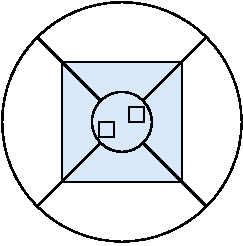
\includegraphics[width=0.60\linewidth]{img/wave_scattering/multipatch_coords}
  \caption{Schematic representation of the \texttt{Thornburg04} coordinate system employed in the simulations. Adapted from Ref.~\cite{Reisswig2010}.}
  \label{fig:wave_scattering_multipatch_coords}
\end{figure}

To preserve the structure of the evolution equations, \texttt{Llama} employs both \textit{local} and \textit{global} coordinate systems. Equations and derivatives are consistently expressed in terms of their respective patch-local coordinates, enabling the use of standard forms of equations and approximations for derivative operators. However, \texttt{Llama} internally stores quantities in a Cartesian global coordinate system in which each patch is embedded. To convert local derivatives (and other vector or tensor quantities, if they exist) to this global coordinate system, it is necessary to project each derivative operator using the Jacobians of the coordinate transformations.

Assuming $x^k$ represent the global Cartesian coordinate system and $a^k$ denotes the local coordinates, the construction of the Jacobian $\tens{J}{i}{k} = \partial a^i / x^k$ permits the expression of first and second order derivatives in the global coordinate system as
%
\begin{equation}
  \hat{\partial}_k = \tens{J}{i}{k} \partial_i
  \label{eq:wave_scattering_projection_1}
\end{equation}
%
and
%
\begin{equation}
  \hat{\partial}_i \hat{\partial}_j = \tens{J}{k}{i} \partial_k \left( \tens{J}{l}{j} \right) \partial_l + \tens{J}{k}{i}\tens{J}{l}{j}\partial_k\partial_l,
  \label{eq:wave_scattering_projection_2}
\end{equation}
%
respectively, where $\partial_i$ denotes derivatives with respect to $a^i$ and $\hat{\partial}_i$ denotes derivatives with respect to $x^i$.

It should be noted that, in order to perform the required calculations, not only the Jacobian of local coordinates is necessary, but also the Jacobian derivatives. \texttt{Llama} provides both the components of the Jacobian and its derivatives at each point on the grid during the evolution process so that the user can project the results according to Eqs~\eqref{eq:wave_scattering_projection_1} and \eqref{eq:wave_scattering_projection_2} manually.

Alternatively, \texttt{Llama} provides a convenience \texttt{Thorn} called \texttt{GlobalDerivatives} that automatically performs the projections for the user. However, in our \texttt{Thorn}, we have opted to perform these projections manually, as \texttt{GlobalDerivatives} does not offer a way to directly compute second-order spatial derivatives. Once again, we have employed Wolfram Matheamatica for generating the \texttt{C} code responsible for projecting derivatives into global coordinates.